%!TEX root = ../thesis.tex
%*******************************************************************************
%*********************************** First Chapter *****************************
%*******************************************************************************

\chapter{Introduction}\label{Introduction}  %Title of the First Chapter

\ifpdf
    \graphicspath{{Chapter1/Figs/Raster/}{Chapter1/Figs/PDF/}{Chapter1/Figs/}}
\else
    \graphicspath{{Chapter1/Figs/Vector/}{Chapter1/Figs/}}
\fi

\section{Context}
As society continues to expand at an unprecedented pace, the planning of water utilities is becoming increasingly difficult. Misplanning the implementation of these utilities can cause high maintenance costs and in turn cost taxpayers billions of pounds. Presently, the UK's largest water supplier has faced severe financial and operational difficulties attributed to mismanagement and underinvestment \citep{Jones2025}. The company is burdened with nearly £19 billion in debt, with escalating interest costs exacerbating its financial instability. These infrastructure deficiencies have resulted in environmental violations and subsequent fines. In February 2025, the regulator Ofwat launched an investigation into Thames Water, further highlighting the financial and operational repercussions of inadequate planning.\newline
Academic studies have also explored the financial impacts of mismanagement in water utilities. A study published in Environmental Research Letters \citep{Skerker2024} highlights that rising water prices, partly a result of operational inefficiencies, force many households to choose between "us[ing] less water than is healthy, forgo[ing] other essential services, [...] or risking water shutoffs". This situation underscores the broader societal costs of misplanning within water utilities.\newline
Another sector where the planning and building of infrastructure rapidly is critical is in the reconstruction of conflict zones. According to \cite{Tzifakis2013}, rebuilding war-torn areas is a "decade-long effort" dependant upon the scale of destruction, the country's economic situation, and the level of international aid available, which "last[s] [...] for as long as a recipient country is on the media spotlight". Designing systems to plan utility piping for areas such as these could assist with these initiatives and help areas recover rapidly, while international aid remains available. While addressing these issues requires proactive investment in infrastructure, transparent management practices, and effective regulatory oversight, the design and usage of a single application designed for the planning of water utilities infrastructure could solve the issues in infrastructure before they arise or help in rebuilding areas ravaged by conflict.\newline
Solving this is not a trivial problem, when routing water networks to different buildings, it is important to consider a plethora of factors: different planning regulations, different locations, and the different requirements of these different buildings all of which come together to require a bespoke solution for each individual situation. A solution for this problem should consider all these factors as well as many more. Given the progress in the capabilities of technology, it is now possible to construct an algorithm that can calculate the most effective solution to planning water utilities in a given area, while still adhering to these different factors and requirements.

\section{Aim and Objectives}\label{aimsandobjectives}
\subsection{Aim}
\textbf{This project aims to create an application that finds the most optimal solution for piping water utilities in a given area.} This will automatically plot the optimal route for water piping – using an optimisation algorithm – between all the given buildings and water sources in an area. The application will feature the ability to account for spatial constraints, the individual requirements of each building – such as the water pressure a building requires - and will have the capacity to account for local planning regulations. The problem will be solved mathematically, using the different requirements as mathematical constraints upon the algorithm. This will overcome the limitations of other programs by creating a dynamic application that can be adapted to any regulatory need.

\subsection{Objectives}\label{objectives}
\begin{enumerate}
    \item Research and identify how water distribution systems function and the standards by which they are laid out to gain a better understanding of these systems. The understanding of distribution systems will directly determine how the algorithm lays out piping systems.
    \item Research optimisers and choose an optimiser to use. Finding the most efficient optimiser to solve the non-linear problem given enhances the quality of the solution and decreases the time the solution takes to produce. In the context of my problem, this will allow me to find the best solution as quickly and efficiently as possible.
    \item Devise a list of functional and non-functional requirements for the theorised application; guided by findings from the prior research.
    \item Produce a mathematical formulation of the problem - using the different requirements (regulatory or otherwise) as mathematical constraints. This will make the problem solvable for the framework and define success for the framework mathematically. This will be used within the optimiser to find the optimal solution to the problem.
    \item Create any classes that may be required (buildings, sources etc.) – this will allow me to create class representations of these physical objects.
    \item Create a GUI that allows the new classes and features to be viewed.
    \item Implement the mathematical formulation into the optimiser as a series of constraints. These will be expressed using linear or integer programming. The optimiser will then use these constraints, along with the objective function, to find the most efficient and valid network configuration.
    \item Iteratively refine the algorithm based on test results, ensuring that it consistently produces valid and optimal solutions, ensuring to update the algorithms appropriately to fix any errors or edge cases.
\end{enumerate}



\section{Project Plan}
The project will begin with comprehensive research of water distribution systems to develop a strong foundational understanding of their structure and challenges. Following this, various existing approaches to solving this, or similar, problems will be critically evaluated to identify the most effective applications, technologies, strategies, and methodologies. Based on the insights gained, a mathematical model will be developed to represent the problem. This model will then be implemented in code, incorporating optimisation techniques where appropriate. The final phase of the project will involve thorough testing and validation to assess the performance, accuracy, and robustness of the implemented solution. Although the project will take an agile approach to development\footnote{As covered in Section \ref{approachtodev}.}, a Gantt chart has been devised with an approximate timeline of the work to be carried out.

\begin{figure}[H]
    \centering
    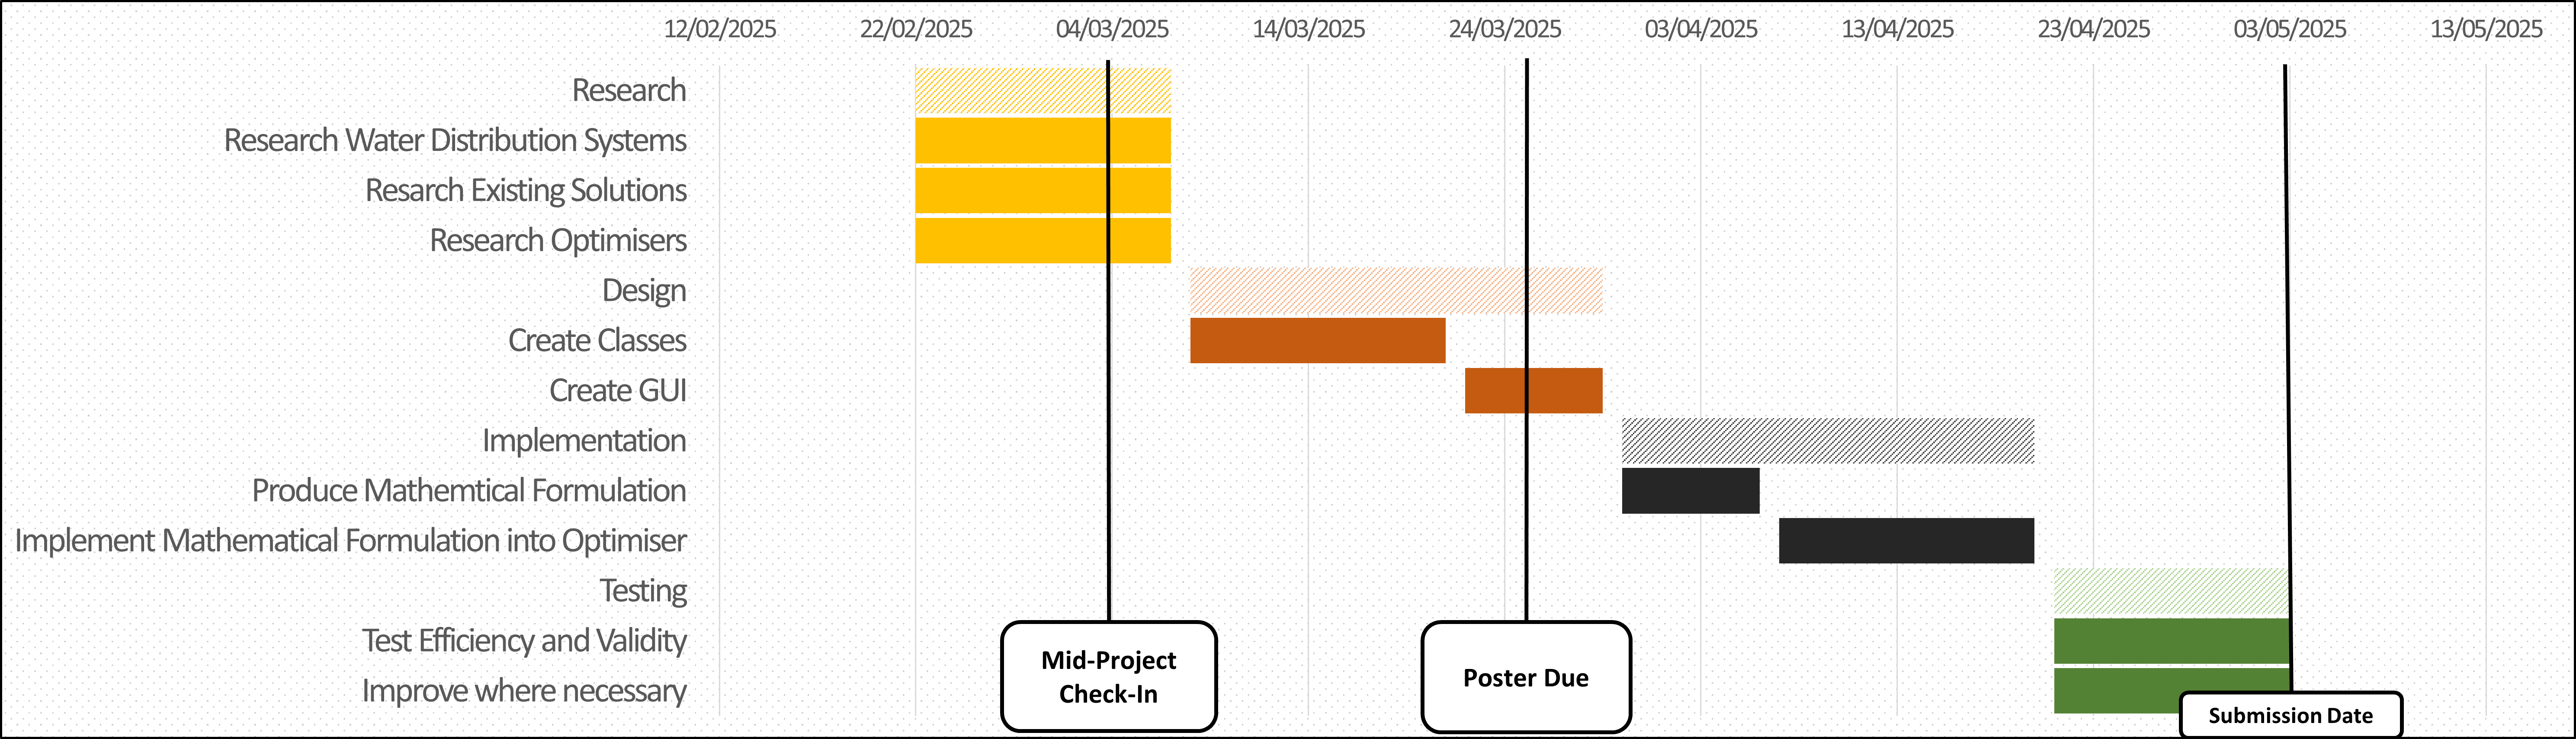
\includegraphics[width=1\linewidth]{Chapter1/Figs/Raster/ganttchart.png}
    \caption{Gantt chart displaying the approximate timeline of works to be carried out.}
    \label{fig:ganttchart}
\end{figure}


\section{Risk Management}
This section will cover the risk associated with delivery and usability of the my project tailored to my objectives.

\begin{longtable}{l p{4.5cm} c c p{4.5cm}}
\caption{Risk Management} \label{table:riskmanagementtable} \\
\toprule
Risk ID & Risk & Likelihood & Impact & Mitigation Strategy\\
\midrule
\endfirsthead

\multicolumn{5}{c}{{\bfseries \tablename\ \thetable{} -- continued from previous page}} \\
\toprule
Risk ID & Risk & Likelihood & Impact & Mitigation Strategy\\
\midrule
\endhead

\midrule \multicolumn{5}{r}{{Continued on next page}} \\
\endfoot

\bottomrule
\endlastfoot

\multicolumn{5}{c}{\textbf{Research \& Mathematical Modelling Risks}} \\
R1 & Incomplete understanding of flow network optimisation models & Medium & High & Conduct thorough research on water distribution systems and network flow.\\
R2 & Mathematical model becomes infeasible (has no solution) under certain input conditions (e.g. not enough water around a circuit) & High & Low & Provide user-friendly diagnostics and inform the user when this is the case\\
R3 & Difficulty translating real-world requirements into mathematical constraints & High & Medium & Begin with a simplified model and perform iterative improvements.\\
\midrule

\multicolumn{5}{c}{\textbf{Technical Design \& Implementation Risks}} \\
R4 & Complexity of integrating optimiser with live UI updates & High & High & Begin with a terminal output in initial testing and iteratively update to a full GUI\\
R5 & Lack of prior experience with Java GUI and Optimisation Frameworks & High & High & Allocate time for learning and focused prototyping.\\
R6 & Problem is NP-hard in Nature and will require intensive calculations to compute the solution leading to long runtimes. & High & Medium & Allow for long runtimes or use sophisticated hardware\\ 
\midrule

\multicolumn{5}{c}{\textbf{Project Management \& Scope Risks}} \\
R7 & Over-scoping (e.g. adding unnecessary features like advanced hydraulics) & Low & Medium & Define clear Functional Requirements.\\
R8 & Lack of clear documentation during development & Low & Low & Comment extensively during prototyping. Schedule regular review checkpoints.\\
\midrule

\multicolumn{5}{c}{\textbf{User Interaction \& Usability Risks}}\\
R9 & Optimisation results may be hard to interpret & Medium & Medium & Use visual overlays e.g. arrows\\
R10 & Error Messages or failures aren't user-friendly & High & Medium & Implement robust error handling. Display errors in the UI rather than console.\\
\end{longtable}


\section{Dissertation Structure}
The following sections of this dissertation outline the steps taken during development chronologically and will consist as follows. Section \ref{Background} will outline the background research performed before modelling development took place. Section \ref{Modelling} will outline the mathematical modelling, and associated research, that took place synchronously with the code implementation outlined in Section \ref{implementation}. Section \ref{Evaluation} will evaluate the final project against the Requirements to be outlined in Section \ref{systemrequirements}. Finally, the conclusion in Section \ref{conclusion} will offer a summary of the project and the potential next steps. 

